% Copyright (c) 2001. David Harrison. All rights reserved.
% Copyright (c) 2003. David Harrison. All rights reserved.
\documentclass[11pt]{article}
%\usepackage{psfig,fullpage,amstext,program}
\usepackage{fullpage,amstext,program,fancybox,latexsym,graphicx}
\textwidth 6.5in
\textheight 8.7in
\setlength{\topmargin}{-1.25in}
%\oddsidemargin -0.1in
%\topmargin -0.25in
\topmargin 0.25in

\begin{document}

%\newenvironment{inventor}{\begin{verse}}{\end{verse}}
%\newcommand{\rlimit}{\ensuremath{\rho}}               % rate limit.
%\newcommand{\excess}{\ensuremath\mathrm{excess} }     % excess.
%\newcommand{\markrate}{\ensuremath{\mathrm{markrate}} }

\title{RPI \verb|ns-2| Graphing and Statistics Package\\
       User Manual and Tutorial}
\author{David Harrison \\
        RPI CS Department\footnote{I have graduated from RPI. Further maintenance and development is being done via Source Forge. http://www.sourceforge.net/projects/ns2graph}}

\maketitle

\begin{abstract}
This user manual contains an installation guide and a short
tutorial for the RPI graphing tools for ns.
\end{abstract}

%\tableofcontents

\section{Introduction}

The RPI ns-2 Graphing and Statistics Package\footnote{Since the name
``RPI ns-2 Graphing and Statistic Package is bulky, we use the
terms ``RPI graph package'' and ``graph package'' interchangeably with
the full name.} provides a set of classes for generating commonly used
plots and gathering commonly important statistics.  The graph package
abstracts data collection from rendering.  Each graph object
instantiates a set of data collection objects which are attached to
components in a network topology, as the simulation runs the data
collection objects collect data often outputting the data to an
intermediate file.  After simulation, the graph object conforms the
data to a canonical format and then sends it to a PlotDevice for
rendering.  By substituting plot devices, the user can cause the same
graph to be output to a window or a file using gnuplot, fig, xgraph,
xdvi, ghostview, or acroread.  In Figure~\ref{PlotDeviceFigure} we
show a utilization graph that collects data from a link in an ns
simulation and then outputs to a gnuplot plot device.  The gnuplot plot
device translates the data and commands from the utilization graph
into gnuplot commands.  The gnuplot application then generates an
encapsulated postscript file.  Other scenarios include rendering a
graph with multiple plot devices for example to generate a postscript
file while simultaneously displaying the data in an X window using
xgraph.  Or multiple graphs may be output to the same acroread plot
device so that the graphs appear in a single acroread window in the
given order.

\begin{figure}
\begin{tabular}{cc}
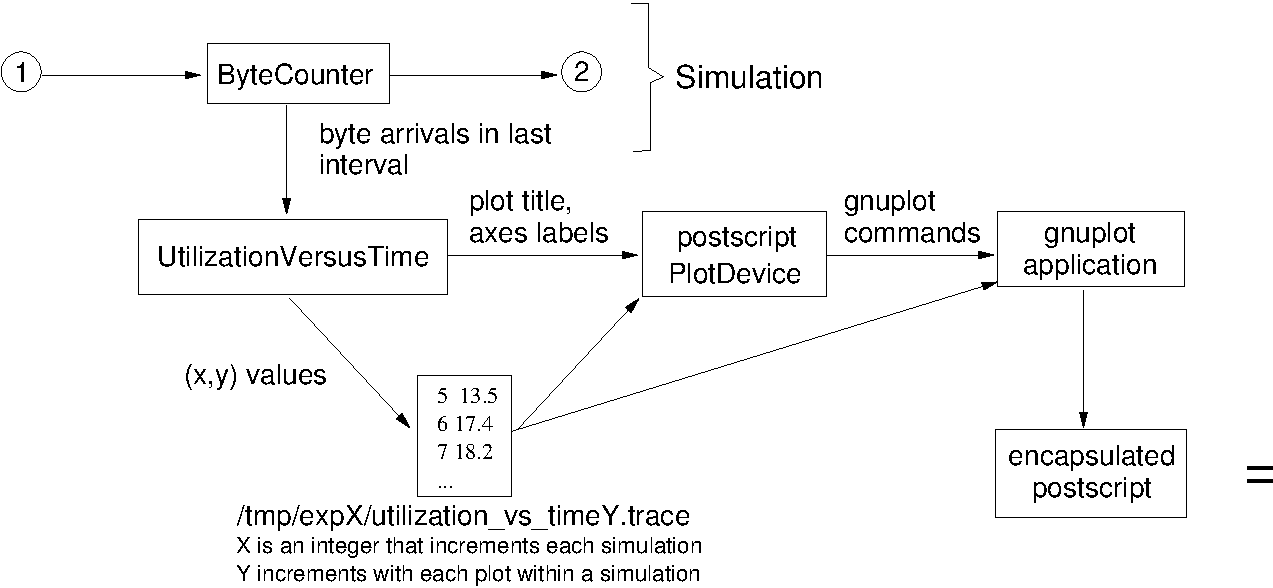
\includegraphics[width=5in]{plot_device} &
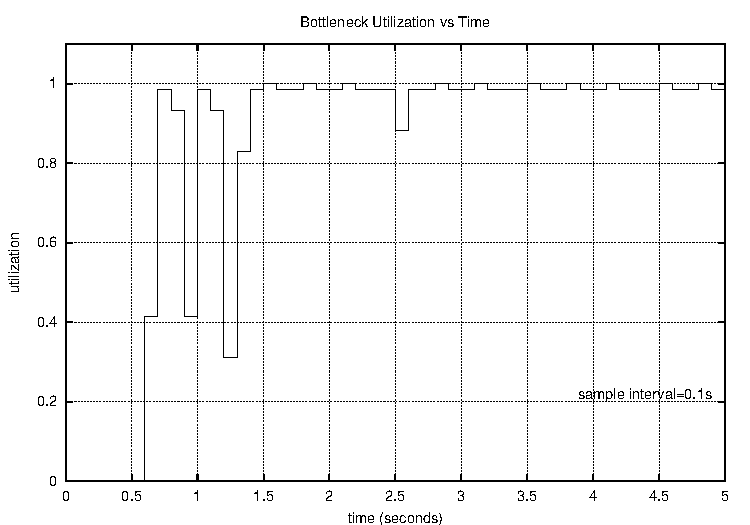
\includegraphics[width=1.25in]{utilization-vs-time}
\end{tabular}
\caption{UtilizationVersusTime Graph outputting via postscript PlotDevice}
\label{PlotDeviceFigure}
\end{figure}

\section{Installation}

Presumably you already have the distribution and have installed
ns-2.   The graph package has been tested with ns-2.1b9a, ns-2.26, 
and ns-2.28.  There may be incompatibilities with 
other ns versions.  If you have not downloaded the graph package then get it
from

% The graph package has been tested with ns-2.1.b5,
%ns-2.1b9a, ns-2.26, ns-2.27, and ns-2.28.  There may be incompatibilities with 
%other ns versions.  If you have not downloaded the graph package then get it
%from

\verb|http://www.ecse.rpi.edu/~harrisod/graph.html|.
\vspace{0.1in}

The graph package comes with an \verb|install| script, which is found in the
root of the directory of the distribution.  This \verb|install| script will
help you through the installation process.  However, it is not fully
automatic.  You will have to edit your shell initialization script
(e.g., .bashrc) and the NS Makefile manually.  The install script will
prompt you when this is necessary.

To unpack the distribution and to run the \verb|install|
script enter

\begin{verbatim}
  > gunzip graph-v6.x.tar.gz
  > tar -xf graph-v6.x.tar
  > cd graph-v6.x
  > ./install
\end{verbatim}

\noindent where $x$ is the minor version number of the graph package.

Should the install script fail you may use the manual install
procedure given in the next section.

\section{Manual Installation}

The following steps are the same as those taken by \verb|install|:

\begin{enumerate}

\item{In order for the graph package to function, you must define two
environment variables: the \verb|NS| environment variable must point
to the root of the \verb|ns| source code tree, and the \verb|NSVER|
environment variable must contain the ns version number (e.g.,
ns-2.1b9a has version ``2.1b9a'').  If you are using bash then add
adding the following to your \verb|.bashrc| file}

\begin{verbatim}
  export NS=/home/harrisod/ns-allinone-2.28/ns-2.28
  export NSVER=2.28
\end{verbatim}

\noindent but change \verb|/home/harrisod| to the appropriate path 
and \verb|NSVER| to reflect the appropriate NS version number.

\item{Make a backup of your \verb|ns| source code tree (i.e.,
\verb|$NS|) before attempting this installation.}

\item{If you have an earlier version of the graph package then remove it 
      as follows}

\begin{verbatim}
  > cd $NS
  > rm -r rpi
  > rm -r tcl/rpi
\end{verbatim}

\item{Move directories from the distribution into your \$NS distribution.}
 
\begin{verbatim}
  > cp -r rpi $NS
  > cp -r tcl/rpi $NS/tcl/rpi
  > cd $NS
\end{verbatim}

\item To configure the paths to the applications used by the graph package
run the configure.tcl script in \$NS/tcl/rpi,

\begin{verbatim}
  > cd $NS/tcl/rpi
  > ns $configure.tcl
\end{verbatim}

This script will look for the following applications:

\begin{itemize}
  \item \verb|nam|,
  \item \verb|acroread|,
  \item \verb|epstopdf|,
  \item \verb|ghostview|, 
  \item \verb|gnuplot|,
  \item \verb|latex|,
  \item \verb|pdflatex|,
  \item \verb|xdvi|,
  \item and \verb|xgraph|.
\end{itemize}

In some cases, the script will also look for alternate applications.
For example in Linux, \verb|evince| can display both postscript and
pdf files, and thus can be used in place of ghostview and acroread.

\noindent
\verb|nam| comes with ns-2, is necessary to run network animations,
and is used in some of the examples provided with this package (see
the examples directory in the root directory of the graph
distribution).  The remaining applications are used in the process of
creating graphs.  Not all of the applications are necessary to use the
graph package though some PlotDevice classes will not function.  See
Table~\ref{PlotDevicesTable} for the list of PlotDevice classes and
the dependencies between these classes and the applications.


\item{Insert the following lines in your \verb|ns| Makefile}

\begin{verbatim}
  [...]
  INCLUDES= \
      -I.  -Irpi \
  [...]
  OBJ_CC= \
  [...]
	rpi/byte-counter.o rpi/delay-monitor.o rpi/file-tools.o \
        rpi/rate-monitor.o rpi/rpi-flowmon.o rpi/rpi-queue-monitor.o \
  [...]      
\end{verbatim}

Here ``\verb|INCLUDES= \|'' and ``\verb|OBJ_CC= \|'' should
already appear in your Makefile.  ``\verb|[...]|'' refers to an omission
of lines already appearing in your Makefile.

\item{Rebuild \verb|ns|}

\begin{verbatim}
  > cd $NS
  > rm gen/* 
  > make depend
  > make
\end{verbatim}

%Problems often arise in this last step.  If the code fails to compile then see 
%Section~\ref{BuildProblemsSection}.

\item{Test \verb|ns|}

Change to the directory \$NS/tcl/rpi/tests.  Type 
  \begin{verbatim}
    run-test-suite.sh
  \end{verbatim}
\end{enumerate}

This will test the RPI Graphing and Statistics package.  You should
see the following output:

\begin{verbatim}
      script-tools.tcl Test:  PASSED all 17 tests.
      ByteCounter Test:       PASSED
      DelayMonitor Test:      PASSED all 6 tests.
      DelayMonitor Garbage Collection Test :  PASSED
      file-tools.tcl Test:    PASSED
      RPIQueueMonitor Tests:  PASSED all 24 tests.
      link-stats Tests:       PASSED all 59 tests.
\end{verbatim}

After the text above, the test suite calls graph\_test/graph-test.tcl,
which generates a set of graphs and displays them using a variety of
plot devices.  

Carefully inspect the generated plots for correctness against the
plots bearing the label ``Comparison Graph.'' Because of the visual
nature of the graphing tools and slight differences between versions
of the various graphing applications, we found that the only reliable
way to test the PlotDevice classes was through visual
inspection.  NOTE: That your output may not look exactly the same as
the provided comparison graphs.  Look for differences in content rather
than small differences in presentation (e.g., ignore font
differences).

%\section{Build Problems}\label{BuildProblemsSection}
%
%\begin{itemize}
%
%\item{Cannot find hash\_map include file}
%  \begin{verbatim}
%    rpi/delay-monitor.h:13:20: hash_map: No such file or directory
%  \end{verbatim}
%
%  This error can arise only if you edit the graph_config.h file and
%  uncomment DELAY_MONITOR_USER_HASH_MAP.  By default, the graph
%  package
%
%  \verb|hash\_map| is not part of the C++ standard STL.  It is however
%  part of the original RPI, HP, and SGI implementations of STL.
%  An implementation of \verb|hash_map| is available in Linux.
%  On my system it is found in 
%
%  \begin{verbatim}
%    /usr/include/c++/3.2/ext/hash_map
%  \end{verbatim}
%
%  The directory may differ on your system.  Once you have located
%  \verb|hash_map|, add the directory to the \verb|INCLUDES| line
%  in the Makefile as is done below:
%
%  \begin{verbatim}
%  INCLUDES = \
%          -I.  -Irpi -Ibass \
%          -I/usr/include/c++/3.2/ext/ \
%  [...]
%  \end{verbatim}
%
%\item{Failed to compile hash\_map}
%  \begin{verbatim}
%    rpi/delay-monitor.h:38: ISO C++ forbids declaration of 
%    `hash_map' with no type
%  \end{verbatim}
%
%  If \verb|GNU_CXX| does not appear in the \verb|DEFINE| line in the
%  \verb|ns| makefile then add it as follows
%
%  \begin{verbatim}
%  DEFINE  = -DGNU_CXX [...]
%  \end{verbatim}  
%
%\end{itemize}

%\clearpage

\section{Tutorial}\label{TutorialSection}

All of these examples assume a working knowledge of \verb|ns|.  If you 
have not created \verb|ns| scripts before then consult the \verb|ns| 
documentation and write a few test scripts before proceeding from here.

Currently the graph package provides the graphs shown in
table~\ref{GraphClassesTable}.

Except for the \verb|XY| class, an instance of any of these classes
gathers statistics directly from an \verb|ns| simulation and renders a plot
when the instance's \verb|plot| member function (i.e., TCL instproc)
is called.  The \verb|XY| class simply allows script writers to
generate a plot from an arbitrary set of $(x,y)$ coordinates.  The
\verb|XY| class represents a way for a script writer to use the
\verb|PlotDevice| classes as a generic interface to a variety of
output devices.

\begin{table}[ht]
\begin{center}
\begin{tabular}{|l|l|}\hline
  CWndVersusTime        & TCP congestion window size versus time \\
  FlowQLenVersusTime    & sampled per-flow queue contribution versus time \\
  PointToPointDelayVersusTime
                        & delay between two points on the network \\
  QDelayVersusTime      & sampled queuing delay versus time \\
  QLenVersusTime        & sampled queue length versus time \\
  RateVersusTime        & arrival rate versus time over constant 
                          interval length \\
  REDQueueVersusTime    & avg queue, instant queue versus time \\
  RTTVarianceVersusTime & TCP variance in round-trip-time versus time \\
  RTTVersusTime         & TCP round-trip time versus time \\
  Sequence              & TCP sequence number versus time \\
  SRTTVersusTime        & TCP smoothed round-trip time versus time \\
  UtilizationVersusTime & utilization versus time over constant 
                          interval length \\
  XY                    & plot $(x,y)$ coordinates from an input file \\\hline
\end{tabular}
\end{center}
\caption{Provided Graph classes}\label{GraphClassesTable}
\end{table}


\subsection{Example 1: Graphing link statistics}

To include the graph package we preface every experiment script with the
following:
  \begin{verbatim}
  source $env(NS)/tcl/rpi/graph.tcl
  \end{verbatim}

The graph package contains several graphs for gathering statistics
about traffic passing through a link including queue length versus time, 
utilization versus time, rate versus time, and queue delay versus time.
In this example we will show how to graph utilization over given
fixed intervals versus time.

Assume we have created a topology with a known bottleneck spanning ns
nodes \verb|n0| and \verb|n1|.  Next we add the lines shown in
figure~\ref{Ex1Figure} to our script.  To collect statistics for our
graph we instantiate a \verb|Graph/UtilizationVersusTime| object.  The
arguments \verb|$n0| and \verb|$n1| tell the graph object to collect
statistics for the link spanning between nodes \verb|n0| and
\verb|n1|.  The 0.1 argument tells the graph object that it should
measure utilization over 0.1 second intervals.  When the simulation
finishes, we call \verb|$util_graph display| to tell the graph object
to show a window containing our utilization versus time plot generated
using \verb|gnuplot|.  We show the complete source code for this script
in \verb|graph-v6.x/examples/ex1.tcl|, and the generated graph in
figure~\ref{Ex1UtilFigure}.

\begin{figure}[!ht]
\begin{center}
\ovalbox{
\begin{minipage}[c]{5.0in}
\begin{verbatim}

[...]
proc finish {} {
  global util_graph
  [...]
  $util_graph display
  exit 0
}
[...]  ;# define nodes n0 and n1 and link spanning them.
# create graph of utilization vs time for link [n0,n1].
set util_graph [new Graph/UtilizationVersusTime $n0 $n1 0.1]

\end{verbatim}
\end{minipage}
}
\end{center}
\caption{Utilization versus time script: ex1.tcl}\label{Ex1Figure}
\end{figure}

\begin{figure}[!ht]
\centerline{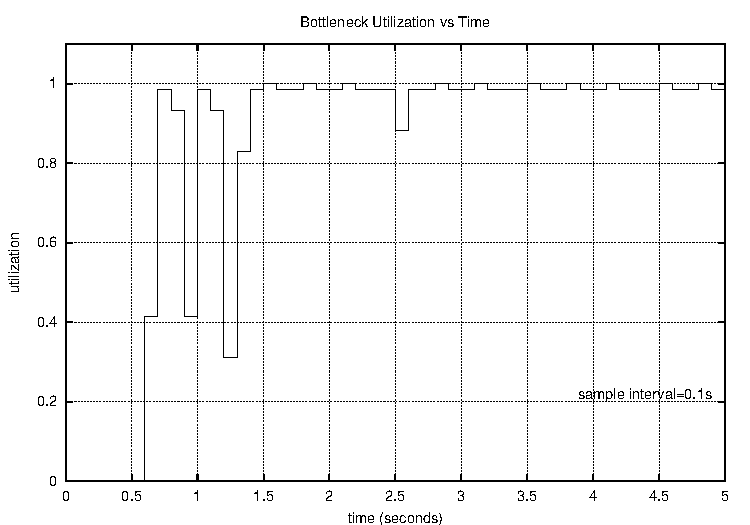
\includegraphics[width=4.5in]{utilization-vs-time}}
\caption{Graph generated by ex1.tcl}\label{Ex1UtilFigure}
\end{figure}

%\begin{figure}[!ht]
%\centerline{\includegraphics[width=3in]{utilization_vs_time0}}
%\includegraphics[width=1]{utilization_vs_time0}
%\caption{Graph generated by ex1.tcl}\label{Ex1UtilFigure}
%\end{figure}

\subsection{Example 2: Outputting to Various Plot Devices}

The graph package can output graphs to windows or files using 
various applications or formats for displaying/saving graphs.  We show
the current set of supported ``plot devices'' in
table~\ref{PlotDevicesTable}.

\begin{table}[ht]
\begin{center}
\begin{tabular}{|l|l|}\hline
  acroread     & \begin{minipage}[c]{4in}
                 \vspace{0.05in}
                 When closed, display all graphs plotted with this 
		 device using acroread.  Uses postscript PlotDevice and the 
                 pdflatex application.
                 \vspace{0.05in}
                 \end{minipage} \\\hline
  fig          & Output to fig file via gnuplot.  \\\hline
  ghostview    & Output eps via gnuplot then display using ghostview \\ \hline
  gnuplot      & Show plot in X window using gnuplot.    \\ \hline
  gnuplot35    & Show plot in X window using gnuplot 3.5 (no comments).
                  \\ \hline
  latex        & \begin{minipage}[c]{4in}
                 \vspace{0.05in}
                 Output to eps file using the postscript PlotDevice
                 and run latex to create a latex file that includes the 
                 graphs.
                 \vspace{0.05in}
                 \end{minipage}  \\ \hline
  pdf          & Output to pdf file from eps using epstopdf.  \\ \hline
  postscript   & Output to encapsulated postscript via gnuplot.  \\ \hline
  postscript35 & Output to eps via gnuplot 3.5 (no comments).  \\ \hline
  xdvi         & \begin{minipage}[c]{4in}
                 \vspace{0.05in}
                 When closed, display all graphs plotted with this
		 device using xdvi.
                 \vspace{0.05in}
                 \end{minipage} \\ \hline
  xgraph       & Show plot in X window using xgraph.  \\ \hline
\end{tabular}
\end{center}
\caption{Supported plot devices}\label{PlotDevicesTable}
\end{table}

In \verb|graph-v6.2/examples/ex2.tcl| we provide an example script
that uses an \verb|xdvi| plot device to display multiple graphs in the
same window in the designated order.  One of the first things we do
in this script is to create a plot device:

\begin{verbatim}
  Graph set plot_device_ [new xdvi]
\end{verbatim}

Here we create an instance of the \verb|xdvi| class and assign it to
the \verb|Graph plot_device_| class member.  Whenever a graph object is
instantiated it by default uses the plot device defined in the 
\verb|Graph plot_device_| class member.  All of the classes can be 
instantiated by passing a plot device object to their respective
\verb|init| instprocs.  This allows you to use a different plot
device for each graph object if you so wish.

We show the relevant snippets from the \verb|ex2.tcl| script in
figure~\ref{Ex2Figure}.  Not shown in figure~\ref{Ex2Figure} we
create a topology containing a bottleneck between nodes \verb|$n0| and
\verb|$n1|.  We then define two TCP connections that pass through the
bottleneck.  The first of these two connections has the TCP agent object
\verb|$tcp0|.  Shown in figure~\ref{Ex2Figure}, we create three graph
objects of which the first two install statistics gathering objects
into the bottleneck link from \verb|n0| to \verb|n1|.  The last graph
object traces the congestion window of \verb|tcp0|.  When the
simulation completes we output each of the graphs to encapsulated
postscript by calling each object's \verb|display| instproc.  Next
we close the plot device causing the plot device to compile a latex
file that references the eps files generated by each graph object.  The
latex compiler outputs an dvi file which the plot device then opens
using xdvi.

\begin{figure}[ht]
\begin{center}
\ovalbox{
\begin{minipage}[c]{5.0in}
\begin{verbatim}

[...]
Graph set plot_device_ [new xdvi]
[...]
proc finish {} {
  global util_graph qlen_graph cwnd0_graph

  $util_graph display
  $qlen_graph display
  $cwnd0_graph display

  [Graph set plot_device_] close

  run-nam
  exit 0
}
[...]  ;# define a bottleneck between n0 and n1.

set util_graph [new Graph/UtilizationVersusTime $n0 $n1 0.1]
$util_graph set title_ "Bottleneck Utilization vs Time"

set qlen_graph [new Graph/QLenVersusTime $n0 $n1]
$qlen_graph set title_ "Bottleneck Queue Length Versus Time"

set cwnd0_graph [new Graph/CWndVersusTime $tcp0]
$cwnd0_graph set title_ "cwnd of flow 0 versus Time"
[...]

\end{verbatim}
\end{minipage}
}
\end{center}
\caption{Example 2: Display multiple graphs using xdvi}\label{Ex2Figure}
\end{figure}

\subsection{Example 3: Outputting Graphs as Files}

Often we want to generate graphs as files for inclusion in a 
report or paper.  In the previous example we showed how to output into
\verb|xdvi|.  In this example we consider outputting to a \verb|fig|
file for later annotation using \verb|xfig|.  With this example we also take
into consideration where generated files are placed in the file
system.

We show code snippets for Example~3 in Figure~\ref{Ex3Figure}.  
Example~3 differs from Example~2 only in that we use a different 
plot device, in this case \verb|fig|, and we explicitly tell
\verb|util_graph| to output to the file named 

\begin{verbatim}
   bneck_util_vs_time
\end{verbatim}

\noindent in the current working directory.  Note that this is not the exact
filename of the output file.  The plot device appends an id unique to the
plot device and then appends a file type extension.  The actual output file's
name is 

\begin{verbatim}
   bneck_util_vs_time_plot1.fig
\end{verbatim}

Note that setting \verb|output_filename_| does not affect the location
of any trace or other temporary files.  All temporary files are by
default written to a temporary directory located in \verb|/tmp/exp|$x$
where $x$ is replaced with the smallest integer that has not already been
used in the naming of another \verb|exp| directory in \verb|/tmp|.
The user can change the default directory by setting
\verb|tmp_directory_| global variable before instantiating any Graph
objects.  However, this is only advisable if the user is sure that the
directory used to store temporary files resides on the same machine
that is executing the script, since writing across a network will not
only slow down the simulation but may adversely affect other users
sharing the network.  

If the user does not set the \verb|output_filename_| data member then
the output file is placed in \verb|tmp_directory_| with a default
name specific to the Graph class.

\begin{figure}[ht]
\begin{center}
\ovalbox{
\begin{minipage}[c]{5.0in}
\begin{verbatim}

[...]
Graph set plot_device_ [new fig]
[...]
set util_graph [new Graph/UtilizationVersusTime $n0 $n1 0.1]
$util_graph set title_ "Bottleneck Utilization vs Time"
$util_graph set output_filename_ "bneck_util_vs_time"
[...]

\end{verbatim}
\end{minipage}
}
\end{center}
\caption{Example 3: Outputting Graphs to Files}\label{Ex3Figure}
\end{figure}

\subsection{Example 4: Multiple Plot Devices}

Note that the caller can output the same graph object to both a file
and a window by using two plot devices.  In \verb|ex4.tcl| we use xgraph
and postscript to generate encapsulated postscript while displaying
the graph using xfig.  We show the relevant code snippet in
Figure~\ref{Ex4Figure}.  Notice that we do not call the ``display''
instance procedure on the graph object.  The graph's ``display''
method plots using the default PlotDevice.  Instead we call the plot
device directly using its ``plot'' instproc, and we pass the graph
to the plot device.

Note that often times there is little need for more than one plot
device since plot devices create intermediate files of the desired
type (e.g., xdvi creates encapsulated postscript files for each graph).  
Multiple plot devices is more useful when the desired file type
is not generated as an intermediate file when displaying the graph in a
window as in \verb|ex4.tcl|.

\begin{figure}[ht]
\begin{center}
\ovalbox{
\begin{minipage}[c]{5.0in}
\begin{verbatim}

[...]
proc finish {} {
  [...]
  set xgraph_plotter [new xgraph]
  set eps_plotter [new postscript]
  $xgraph_plotter plot $util_graph
  $eps_plotter plot $util_graph

  $xgraph_plotter close
  $eps_plotter close
  [...]
}
[...]
set util_graph [new Graph/UtilizationVersusTime $n0 $n1 0.1]
$util_graph set title_ "Bottleneck Utilization vs Time"
$util_graph set output_filename_ "bneck_util_vs_time"
[...]

\end{verbatim}
\end{minipage}
}
\end{center}
\caption{Example 4: Output to a file and to an X window using xgraph}\label{Ex4Figure}
\end{figure}

\subsection{Example 5: Using overlays}

With all of the graph classes in the graph package you can overlay the
data from one plot on top of another.  For example, in this section we
show how to plot congestion window versus time for two TCP connections
in the same plot.  In Figure~\ref{ExOverlayFigure} we show a TCL snippet
that calls \verb|overlay| in the \verb|finish| procedure to combine
\verb|cwnd0_graph| and \verb|cwnd1_graph|.

\begin{figure}[ht]
\begin{center}
\ovalbox{
\begin{minipage}[c]{5.0in}
\begin{verbatim}

[...]
proc finish {} {
  [...]
  $cwnd0_graph overlay $cwnd1_graph "TCP 1 " "TCP 0 "
  $cwnd0_graph display
  [...]
}
[...]
set cwnd0_graph [new Graph/CWndVersusTime $tcp0]
set cwnd1_graph [new Graph/CWndVersusTime $tcp1]
$cwnd0_graph set title_ "cwnd of flows 0 and 1 versus Time"
[...]

\end{verbatim}
\end{minipage}
}
\end{center}
\caption{Example 5: overlay cwnd for connection 1 on cwnd graph for connection 0.}\label{ExOverlayFigure}
\end{figure}

\begin{figure}[!ht]
\centerline{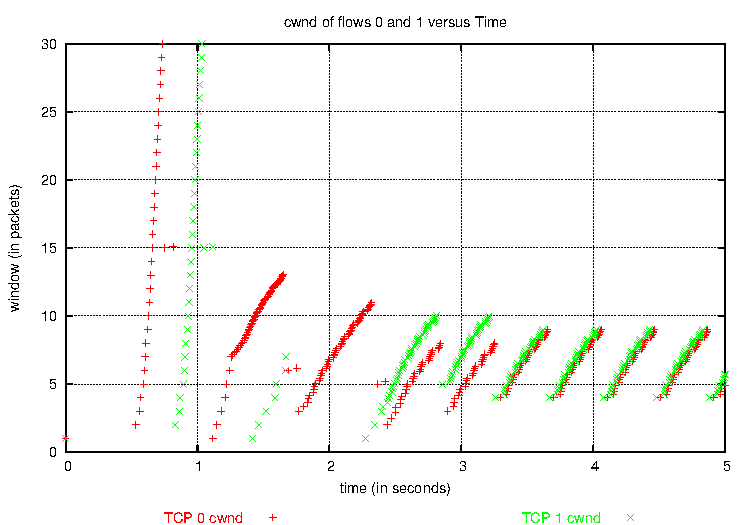
\includegraphics[width=4.5in]{tcp-cwnd-vs-time}}
\caption{Graph generated by ex5.tcl}\label{ExOverlayPlotFigure}
\end{figure}

The act of overlaying plot $x$ onto plot $y$ by calling
\verb|$y overlay $x| causes $x$'s \verb|prepare| method to be called,
but it does not otherwise affect $x$.  However, $y$ copies $x$'s data
set objects.  $y$ keeps its own data sets.  However, $y$ and $x$ share
$x$'s data files for the data sets obtained from $x$.  $y$ retains its
basic appearance.  Appling an overlay does not change $y$'s title,
axis labels, caption, comment, over horizontal lines.  If the x or y
axis ranges have been defined then they also do not change.  However,
if the x or y axis ranges have not been explicitly set then the
underlying plot device may modify the axes ranges to display all data
sets.  For example, gnuplot and xgraph scale x and y axes automatically
when the ranges are not explicitly provided.


The \verb|overlay| procedure takes three arguments.  The first argument
specifies the graph that will be overlayed.  The second argument
specifies a prefix that is prepended to all data set names (i.e., the
names that appear in the key) for the data sets obained from the graph
specified in the first argument.  In Figure~\ref{ExOverlayFigure}, ``TCP 1
`` is prepended to connection 1's cwnd label in the key.  The third
argument specifies a prefix that is prepended to all of the data sets
in the graph whose \verb|overlay| procedure is being called.  In
Figure~\ref{ExOverlayFigure}, ``TCP 0 `` is prepended to connection 0's cwnd
label in the key.  The last two arguments are optional.


\subsection{Example 6: Bottleneck link statistics}

We now move on to demonstrating how to collect statistics using
the statistics functions included with the graph package.  
The objective of these statistics gathering tools is to simplify
statistics gathering over the standard methods provided by 
\verb|ns|.  

To include the link statistics gathering functions do the following:

\begin{verbatim}
      source $env(NS)/tcl/rpi/link-stats.tcl
\end{verbatim}

To begin gathering statistics on a link spanning from nodes \verb|n0|
to \verb|n1|, do the following:

\begin{verbatim}
      set stats [new LinkStats $n0 $n1]
\end{verbatim}

We show code snippets from \verb|examples/ex5.tcl| in
figure~\ref{Ex6Figure}.  The calls to \verb|get-utilization|,
\verb|get-mean-queue-delay|, and \verb|get-packet-arrivals| returns
the link statistics gathered from the moment the link-stats object was
instantiated.  In this case, that means reporting statistics gathered
from the beginning of the simulation.  There are many more statistics
we could report by simply calling any of the instance procedures in
table~\ref{LinkStatsTable}.

\begin{figure}[ht]
\begin{center}
\ovalbox{
\begin{minipage}[c]{5.0in}
\begin{verbatim}

[...]
proc finish {} {
  global n0 n1 tcp0 tcp1 stats

  # output link statistics
  puts "Bottleneck statistics: "
  puts "Utilization: [$stats get-utilization]"
  puts "Number of drops: [$stats get-packet-drops]"
  puts "Mean queue delay [$stats get-mean-queue-delay]"
  puts "Number of arrivals [$stats get-packet-arrivals]"
  [...]
}
[...]  ;# create topology w/ bottleneck between n0 and n1.

set stats [new LinkStats $n0 $n1]
[...]

\end{verbatim}
\end{minipage}
}
\end{center}
\caption{Example 6: Gathering link statistics}\label{Ex6Figure}
\end{figure}


If you wish to gather statistics starting from some time into the
simulation then simply instantiate the \verb|LinkStats| object at that
time.  If you want to gather statistics over consecutive time intervals
then you can reset the link statistics at the end of each time interval by
calling the \verb|LinkStats reset| instance procedure.  If you want to
collect a link's statistics for overlapping intervals then create two
\verb|LinkStats| objects each at a time when you want to begin
collecting statistics then retrieve the statistics at the end
of their respective intervals.  Installing more than one
\verb|LinkStats| object on a link is particularly useful when you 
want to record statistics for the whole simulation as well as 
for the steady-state (i.e., skipping some time to eliminate 
initial transients).

\begin{table}[ht]
\begin{center}
\begin{tabular}{|l|l|}\hline
\verb|init| $n0$ $n1$ [$qmon$] &
  \begin{minipage}[c]{4in}
  \vspace{0.05in}
  Instantiates a LinkStats object spanning between $n0$ and $n1$.
  You must have previously created these two nodes and a link
  spanning these nodes.  More than one LinkStats object can
  span between $n0$ and $n1$.  By default the LinkStats object
  uses an instance of the \verb|RPIQueueMonitor| class to
  collect statistics.  You can install your own queue monitor
  using the optional third argument.
  \vspace{0.05in}
  \end{minipage} \\ \hline
  
\verb|reset|  &
  \begin{minipage}[c]{4in}
  \vspace{0.05in}
  resets all statistics to the initial state.
  \vspace{0.05in}
  \end{minipage} \\ \hline
  
\end{tabular}
\end{center}
\caption{Special instance procedures for LinkStats}
\end{table}


\begin{table}[ht]
\begin{center}
\begin{tabular}{|l|l|}\hline
\verb|get-utilization|         & 
  \begin{minipage}[c]{3.5in}
  \vspace{0.05in}
  Returns the link utilization as the number of bytes departing 
  the queue as the number of bytes that could have departed the queue.
  \vspace{0.05in}
  \end{minipage} \\ \hline

\verb|get-packet-utilization| \emph{avgpktsz}& 
  \begin{minipage}[c]{3.5in} 
  \vspace{0.05in}
  Returns the link utilization as the number of packets that departed
  the bottleneck link times the average packet size over the number of
  average sized packets that could have departed the link.  The
  argument specifies the average packet size.
  \vspace{0.05in}
  \end{minipage} \\ \hline

\verb|get-throughput | &
  \begin{minipage}[c]{3.5in}
  \vspace{0.05in}
  Returns the number of byte arrivals at the tail of the queue * 8 
  over time.
  \vspace{0.05in}
  \end{minipage} \\ \hline

\verb|get-packet-arrivals| &
  \begin{minipage}[c]{3.5in}
  \vspace{0.05in}
  Returns the number of packet arrivals at the tail of the queue.
  \vspace{0.05in}
  \end{minipage} \\ \hline

\verb|get-byte-arrivals| &
  \begin{minipage}[c]{3.5in}
  \vspace{0.05in}
  Returns the number of byte arrivals at the tail of the queue.
  \vspace{0.05in}
  \end{minipage} \\ \hline

\verb|get-packet-drops| &
  \begin{minipage}[c]{3.5in}
  \vspace{0.05in}
  Returns the number of packets dropped.
  \vspace{0.05in}
  \end{minipage} \\ \hline

\verb|get-byte-drops| &
  \begin{minipage}[c]{3.5in}
  \vspace{0.05in}
  Returns the number of bytes dropped.
  \vspace{0.05in}
  \end{minipage} \\ \hline

\verb|get-packet-departures| &
  \begin{minipage}[c]{3.5in}
  \vspace{0.05in}
  Returns the number of packets that departed the queue.
  \vspace{0.05in}
  \end{minipage} \\ \hline

\verb|get-byte-departures| &
  \begin{minipage}[c]{3.5in}
  \vspace{0.05in}
  Returns the number of bytes that departed the queue.
  \vspace{0.05in}
  \end{minipage} \\ \hline

\verb|get-mean-queue-delay| &
  \begin{minipage}[c]{3.5in}
  \vspace{0.05in}
  Returns the mean delay experienced by packets transiting the queue.
  \vspace{0.05in}
  \end{minipage} \\ \hline

\verb|get-queue-delay-variance| &
  \begin{minipage}[c]{3.5in}
  \vspace{0.05in}
  Returns the variance in delay experienced by packets transiting 
  the queue.
  \vspace{0.05in}
  \end{minipage} \\ \hline

\verb|get-queue-delay-stddev| &
  \begin{minipage}[c]{3.5in}
  \vspace{0.05in}
  Returns the standard deviation in delay experienced by packets 
  transiting the queue.
  \vspace{0.05in}
  \end{minipage} \\ \hline

\verb|get-mean-packet-queue-length| &
  \begin{minipage}[c]{3.5in}
  \vspace{0.05in}
  Returns the mean packet queue length.  This is not the same as the
  mean queue length seen by an arriving packet which would not take
  into account idle times in the mean.
  \vspace{0.05in}
  \end{minipage} \\ \hline

\verb|get-mean-byte-queue-length| &
  \begin{minipage}[c]{3.5in}
  \vspace{0.05in}
  Same as \verb|get-mean-packet-queue-length| except the result is 
  returned in units of bytes.
  \vspace{0.05in}
  \end{minipage} \\ \hline

\verb|get-max-packet-queue-length| &
  \begin{minipage}[c]{3.5in}
  \vspace{0.05in}
  Returns the maximum queue length in packets.
  \vspace{0.05in}
  \end{minipage} \\ \hline

\verb|get-max-byte-queue-length| &
  \begin{minipage}[c]{3.5in}
  \vspace{0.05in}
  Returns the maximum queue length in bytes.
  \vspace{0.05in}
  \end{minipage} \\ \hline

\verb|get-min-packet-queue-length| &
  \begin{minipage}[c]{3.5in}
  \vspace{0.05in}
  Returns the minimum queue length in bytes.  Typically this would be
  zero except when measured over some small interval.
  \vspace{0.05in}
  \end{minipage} \\ \hline

\verb|get-min-byte-queue-length| &
  \begin{minipage}[c]{3.5in}
  \vspace{0.05in}
  Same as \verb|get-min-byte-queue-length| except the result is
  returned in units of bytes.
  \vspace{0.05in}
  \end{minipage} \\ \hline

\end{tabular}
\end{center}
\caption{LinkStats statistics instance procedures}\label{LinkStatsTable}
\end{table}

We provide the code for this complete example in
\verb|graph-v6.2/examples/ex6.tcl|.

%\clearpage
\subsection{Example 7: TCP statistics}

The most direct way to obtain TCP statistics is to simply 
query the bound variables defined for the Agent/TCP class.  For
example, if we define a TCP agent \verb|$tcp0| then we can do
the following without extending \verb|ns-2|:

\begin{verbatim}
    puts "Number of data packets transmitted by flow 0: \
      [$tcp0 set ndatapack_]"
    puts "Number of data packets transmitted by flow 1: \
      [$tcp1 set ndatapack_]"
    puts "Retransmission timeouts for flow 0: \
      [$tcp0 set nrexmit_]"
    puts "Retransmission timeout for flow 1: \
      [$tcp1 set nrexmit_]"
\end{verbatim}

When using our TCP statistics gathering functions it is necessary to
include the \verb|tcp-stats.tcl| package.  This loads the definitions
shown in tables~\ref{TCPStatsTable} and~\ref{ListTCPStatsTable}:

\begin{verbatim}
    source $env(NS)/tcl/rpi/tcp-stats.tcl
\end{verbatim}

Then initialize various counters by calling
\verb|init-stats|.  \verb|init-stats| can also be called to simply
reset the the statistics for both our extensions and the statistics
gathered by \verb|ns|.

\begin{verbatim} 
    [...]
    $tcp init-stats
    [...]
\end{verbatim}

At some later time, such as when \verb|finish| is called, 
you can output tcp-statistics as follows:

\begin{verbatim}
    puts "Goodput Variance: \
      [get-goodput-stddev "$tcp0 $tcp1"]"
    puts "Total TCP packets: \
      [get-total-data-packets "$tcp0 $tcp1"]"
\end{verbatim}

In the example above, \verb|get-goodput-stddev| and
\verb|get-total-data-packets| operate on a list of tcp agents.  In this
case returning the standard deviation in goodput and the sum of the
data packets sent respectively across the passed list of agents.
The above examples can be found in \verb|examples/ex7.tcl|.

\begin{table}[ht]
\begin{center}
\begin{tabular}{|l|l|}\hline
\verb|get-useful-packets| & 
  \begin{minipage}[c]{4in}
  \vspace{0.05in}
  Returns the number of packets transmitted containing new data.
  \vspace{0.05in}
  \end{minipage} \\ \hline

\verb|get-useful-bytes| &
  \begin{minipage}[c]{4in}
  \vspace{0.05in}
  Returns the number of bytes transmitted containing new
  data.  The number of useful bytes in each useful packet
  is the packet size minus the TCP and IP headers.  The header size
  is determined by \verb|tcpip_base_hdr_size_| defined in
  \verb|$NS/tcl/lib/ns-default.tcl|.  In ns-2.1b5, 
  \verb|tcpip_base_hdr_size_| is set to 40.
  \vspace{0.05in}
  \end{minipage} \\ \hline

\verb|get-goodput-bps| &
  \begin{minipage}[c]{4in}
  \vspace{0.05in}

  Returns the rate of useful bits transmitted by the network.  Uses
  get-useful-bytes to determine the total number of useful bits.
  Packets that have been lost but not yet detected by the source are
  counted as useful because our measure is based on state maintained
  by the TCP source.  In a long simulation this should have negligible
  impact on the goodput measure.

  \vspace{0.05in} \end{minipage} \\  \hline


\verb|get-goodput| &
  \begin{minipage}[c]{4in}
  \vspace{0.05in}

  Returns goodput in bps over the bottleneck capacity.
  
  \vspace{0.05in}
  \end{minipage} \\ \hline

\verb|get-throughput-bps| &
  \begin{minipage}[c]{4in}
  \vspace{0.05in}
  Returns the throughput in bps.  This counts each retransmission as a separate
  packet.  This differs from get-useful-bytes and get-useful-packets which
  only count the packets sent containing new data.
  \vspace{0.05in}
  \end{minipage} \\ \hline
  
\end{tabular}
\end{center}
\caption{TCP statistics gathering instance procs}\label{TCPStatsTable}
\end{table}

\begin{table}[ht]
\begin{center}
\begin{tabular}{|l|l|}\hline

\verb|get-mean-goodput| $tcplist$ &
  \begin{minipage}[c]{3in}
  \vspace{0.05in}
  Calculates mean goodput in bps across the passed TCP agents 
  (i.e., connections).
  \vspace{0.05in}
  \end{minipage} \\ \hline

\verb|get-goodput-variance| $tcplist$ &
  \begin{minipage}[c]{3in}
  \vspace{0.05in}
  Calculates variance in goodput (bps) across the passed TCP agents
  (i.e., connections).
  \vspace{0.05in}
  \end{minipage} \\ \hline

\verb|get-goodput-stddev| $tcplist$ &
  \begin{minipage}[c]{3in}
  \vspace{0.05in}
  Calculates the standard deviation in goodput in bps across the
  passed TCP agents (i.e., connections).
  \vspace{0.05in}
  \end{minipage} \\ \hline

\verb|get-goodput-cov| $tcplist$ &
  \begin{minipage}[c]{3in}
  \vspace{0.05in}
  Calculates the Coefficient of Variation (C.O.V.) across the passed
  TCP agents.  C.O.V.  is standard deviation over the mean.
  \vspace{0.05in}
  \end{minipage} \\ \hline


\verb|get-total-data-packets| $tcplist$ &
  \begin{minipage}[c]{3in}
  \vspace{0.05in}
  Calculates the sum of the packets sent across the passed TCP agents
  (i.e., connections).
  \vspace{0.05in}
  \end{minipage} \\ \hline

\verb|get-total-retransmitted-packets| $tcplist$ &
  \begin{minipage}[c]{3in}
  \vspace{0.05in}
  Calculates the sum of the packet retransmissions across the passed
  TCP agents (i.e., connections).
  \vspace{0.05in}
  \end{minipage} \\ \hline

\verb|get-total-retransmission-timeouts| $tcplist$ &
  \begin{minipage}[c]{3in}
  \vspace{0.05in}
  Calculates the sum of the retransmission timeouts across the passed
  TCP agents (i.e., connections).
  \vspace{0.05in}
  \end{minipage} \\ \hline

\end{tabular}
\end{center}
\caption{TCP statistics functions operating on lists}\label{ListTCPStatsTable}
\end{table}

\clearpage
\subsection{Example 8: Customizing graph appearance and layout}\label{Ex8Section}

In prior sections we mostly relied on the default behavior of the
Graph and PlotDevice objects.  In this section we explore some of the
options available for affecting the appearance and arrangement of graphs.

First we consider Graph options.  In particular we consider captions,
comments, axes labels, adding horizontal lines and inserting latex in 
the output.

\begin{description}
\item[Title] {To set the title that appears in the plot set the 
  \verb|title_| data member of the graph object.  For example,}

  \begin{verbatim}
    $qlen_graph set caption_ "Bottleneck Queue Length Versus Time"
  \end{verbatim}

\item[Axis Labels] {To set an axis label, set the \verb|ylabel_| or
   \verb|xlabel_| data members of the graph object.  For example,}

  \begin{verbatim}
    $qlen_graph set xlabel_ "Simulation Time (in seconds)"
  \end{verbatim}

\item[Captions] {To incorporate captions, define the \verb|caption_|
  data member of the graph object like follows:}
  \begin{verbatim}
   $qlen_graph set caption_ "Two TCP connections traverse this bottleneck."
  \end{verbatim}

\item[Horizontal Lines] {You can add horizontal lines to any graph by
  calling the \verb|add-hline| instproc.  For example,}

  \begin{verbatim}
    $qlen_graph add-hline 10 "Buffer size"
  \end{verbatim}

  This adds a horizontal line at 10 and adds a entry in the 
  key labelled ``Buffer size.''  This package currently provides
  no method for creating verticle lines.

\item[Comments] {You can add a comment to any graph at a position
  specified using x,y coordinates that each range from 0 to 1.  Note
  that the coordinates are not specified in data units.  (0,0) places
  the comment near the origin, and (1,1) places the comment in the
  upper right-hand corner.  For example, in our queue length graph we
  can add a comment stating that the queue length is instanteous as
  opposed to averaged and place this comment in the upper left-hand
  corner of the plot by doing the following:}

  \begin{verbatim}
    $qlen_graph set comment_ "Instantaneous queue length"
    $qlen_graph set xcomment_ .3
    $qlen_graph set ycomment_ .65
  \end{verbatim}

\item[Axes Ranges] {We can control the range of values on each axes
   in order to zoom in on a region or to improve appearance by setting
   the \verb|xhigh_|, \verb|xlow_|, \verb|yhigh_|, and/or \verb|ylow_|
   data members of the graph object.  If for example, we want to zoom 
   in on the first two seconds of the simulation and we want to 
   extend the upper range of the y-axis so that the buffer size horizontal
   line is not coincident with the top border of the graph, we
   add the following to our script:
  }

  \begin{verbatim}
    $qlen_graph set xhigh_ 2
    $qlen_graph set yhigh_ 11
  \end{verbatim}

\end{description}

We add all of these options together in example 8 as shown in
Figure~\ref{Ex8Figure}.  We show the unadorned graph in 
Figure~\ref{Ex8Graph}(a), and with all of the appearance modifications
in Figure~\ref{Ex8Graph}(b).


\begin{figure}[ht]
\begin{center}
\ovalbox{
\begin{minipage}[c]{5.0in}
\begin{verbatim}
    Graph set plot_device_ [new acroread]
    [...]
    proc finish {} {
      global qlen_graph
      [...]
      $qlen_graph add-hline 10 "Buffer size"
      $qlen_graph set title_ \
        "Bottleneck Queue Length Versus Time"
      $qlen_graph set ylabel_ \
        "Queue Length (in packets)"
      $qlen_graph set xlabel_ "Simulation Time (in seconds)"
      $qlen_graph set caption_ \
        "Two TCP connections traverse this bottleneck."
      $qlen_graph set comment_ \
        "Instantaneous queue length"
      $qlen_graph set xcomment_ .3
      $qlen_graph set ycomment_ .65
      $qlen_graph set xhigh_ 2
      $qlen_graph set yhigh_ 11
      $qlen_graph display
      [...]
    }
    [...]  ;# create topology w/ bottleneck between n0 and n1.
\end{verbatim}
\end{minipage}
}
\end{center}
\caption{Example 8: Customizing graph appearance.}\label{Ex8Figure}
\end{figure}

Assume that we want to juxtapose plots so that more than one appears
on each line (i.e., more than one per row).  We do this by telling the
latex class to generate appropriate latex to fit the desired number of
graphs in each row of output.  For example, if we want 2 graphs per
row we do the following:

  \begin{verbatim}
    latex set n_plots_per_row_ 2
    Graph set plot_device_ [new acroread]
  \end{verbatim}

Above, we set the \verb|latex| class's \verb|n_plots_per_row_| class
variable.  By setting this value before creating the \verb|acroread|
plot device, we ensure that any \verb|latex| object instantiated by
\verb|acroread| as a low-level plotter will set its object data member
\verb|n_plots_per_row_| equal to its class data member of the same
name.

If we want to insert some text anywhere in the output latex, we call
the plot device's \verb|output-latex| instproc.  The text
will appear in order with any plots meaning if we want the text to
appear before any plots then we must call \verb|output-latex| before
calling a graph object's \verb|display| instproc to generate the first
plot.  For example, if we want to add a title to the output latex
file we could do the following:

\begin{verbatim}
  [...]
  set pd [new acroread]
  Graph set plot_device_ $pd
  $pd output-latex \
    {\title{Example 8 Simulation Results}\maketitle}
  [...]
\end{verbatim}

If we want to output some descriptive text in between plots 
we do the following:

\begin{verbatim}
  $qlen_graph plot
  [...]
  $pd output-latex "We now want to generate another plot."
  [...]
  $qlen_graph plot
\end{verbatim}

Unfortunately the \verb|latex| plot device class is not particularly
smart.  It will allow you to output latex at any point even if it
screws up other formatting.  For example, if you are outputing more
than one plot per row, be careful not to insert text in the middle of
a row.  For example, if \verb|n_plots_per_row_| is 2 then only call
\verb|output-latex| after generating an even number of plots.

\begin{figure}
\begin{tabular}{cc}
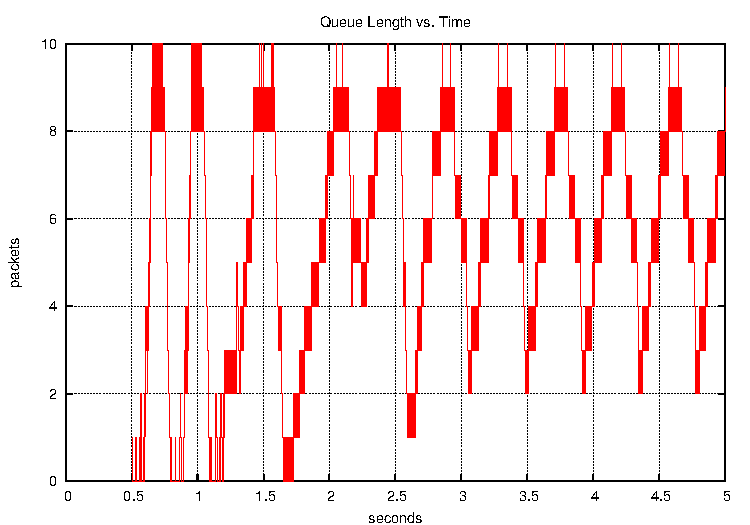
\includegraphics[width=3in]{qlen_vs_time0_plot1} &
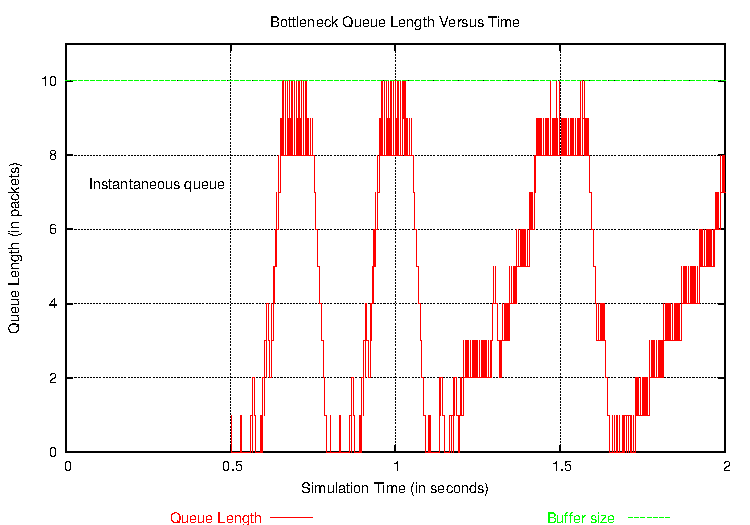
\includegraphics[width=3in]{qlen_vs_time0_plot2} \\
(a) & (b) \\
\end{tabular}
\caption{(a)~shows the graph with default appearance.  (b)~shows the graph
  with modified appearance using the options described in 
  Section~\ref{Ex8Section}.}\label{Ex8Graph}

\end{figure}

Note that not all of these options are supported by all plot devices.
When an option is unsupported, the plot device simply ignores the
option.

\subsection{Example 9: XY Plots}

If all existing graph types do not satisfy your needs, and you just
need to graph something right now as opposed to going through the
overhead of extending the graph package, we suggest using the XY graph
class.  The XY graph class takes as input a text file containing two
white-space delimited columns.  The left column contains X values and
the right column contains Y values.  

For example, when we create an XY graph
\begin{verbatim}
  set xy_graph [new Graph/XY "ex9_thruput_vs_rtpd.txt"]
\end{verbatim}

\noindent that XY graph expects $(x,y)$ coordinates to be output
into a file named \verb|ex9_thruput_vs_rtpd.txt| in a format like

\begin{verbatim}
  16 18530.909090909092
  24 93032.727272727279
  32 149381.81818181818
  ...
\end{verbatim}

\noindent where 16, 24, and 32 are $x$-values and the right column
provides the $y$-values.

In \verb|ex9.tcl|, we show how to use Graph/XY to graph something
that is not provided by a graph within the RPI graph package.  In
this particular example we demonstrate the effect of heterogeneous
round-trip propagation delay on TCP.  It is well-known that 
TCP throughput is roughly inversely proportional to round trip time.

To demonstrate the bias against long round-trip times we first
create a dumbbell topology with $N$ paths each with a different round-trip
propagation delay.

\begin{verbatim}
  for { set i 0 } { $i < $N } { incr i } {
    set s($i) [$ns node]
    set d($i) [$ns node]
  }
  set b0 [$ns node]
  set b1 [$ns node]
  
  # create links.
  for { set i 0 } { $i < $N } { incr i } {
    $ns duplex-link $s($i) $b0 10M [expr 4 * $i]ms DropTail
    $ns duplex-link $b1 $d($i) 10M 4ms DropTail
  }
\end{verbatim}

We create one TCP/Reno connection on each path through the 
dumbbell.

\begin{verbatim}
  for { set i 0 } { $i < $N } { incr i } {
    create-ftp-over-reno $s($i) $d($i) [expr 0.5 * $i] $i] 0
  }
\end{verbatim}
  

We then install link statistics gathering components on each 
of the bottleneck-destination links as follows:

\begin{verbatim}
  for { set i 0 } { $i < $N } { incr i } {
    set lstats($i) [new LinkStats $b1 $d($i)]
  }
\end{verbatim}

When the simulation completes after sufficient time (30 seconds) for the 
simulation to reach steady-state, we read the statistics from the LinkStats
objects and output $(delay,throughput)$ values to the file named 

\begin{verbatim}
  ex9_thruput_vs_rtpd.txt
\end{verbatim}

\noindent by doing 

\begin{verbatim}
  for { set i 0 } { $i < $N } { incr i } {
    set thruput [$lstats($i) get-throughput]
    puts $fp "[expr ($i * 4 + 4 + 4) * 2] $thruput"
  }
\end{verbatim}

We then generate the graph just as we would with any other 
graph, we call the graph's \verb|display| procedure,

\begin{verbatim}
  $xy_graph display
\end{verbatim}

A slightly more complete summary of this script is provided in 
Figure~\ref{Ex9Figure}.  The resulting graph is shown in 
Figure~\ref{Ex9Graph}.  The graph does not show a strictly decreasing 
throughput with increasing round-trip propagation delay, but this could 
be due such factors as synchronization effects because we are using a drop 
tail queue.  The reader could remove synchronization effects by placing
a random dropper like RED at the bottleneck.  We leave this as an
excercise.

\begin{figure}[ht]
\begin{center}
\ovalbox{
\begin{minipage}[c]{5.0in}
\begin{verbatim}

[...]
proc finish {} {
  global xy_graph lstats N

  set fp [open "ex9_thruput_vs_rtpd.txt" "w"]
  for { set i 0 } { $i < $N } { incr i } {
    set thruput [$lstats($i) get-throughput]
    puts $fp "[expr ($i * 4 + 4 + 4) * 2] $thruput"
  }
  close $fp

  $xy_graph display

  [Graph set plot_device_] close
  exit 0
}

set ns [new Simulator]
set xy_graph [new Graph/XY "ex9_thruput_vs_rtpd.txt"]
$xy_graph set title_ \   
  "Connection Throughput versus Round-trip Propagation Delay"
$xy_graph set xlabel_ \
  "Round-trip Propagation Delay (in ms)"
$xy_graph set ylabel_ \
  "Throughput (in bps)"
[...]

\end{verbatim}
\end{minipage}
}
\end{center}
\caption{Example 9: Generate an XY plot to show throughput versus RTPD.}
\label{Ex9Figure}
\end{figure}


\begin{figure}
\centerline{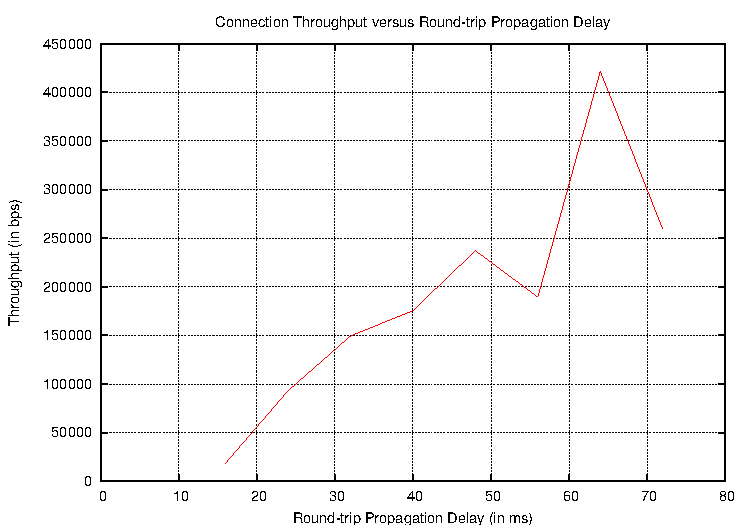
\includegraphics[width=4.5in]{xy_vs_time0_plot1}} 
\caption{XY Graph generated by ex9.tcl showing the bias round-trip propagation delay has on TCP throughput.}\label{Ex9Graph}

\end{figure}

\section{Performance Issues}

When one is running large or long simulations, there are various
considerations to take into account with respect to the tools used for
gathering statistics or generating statistics.  Our tools have been
defined to introduce reasonable overhead, though in some cases
simulation performance constraints may drive one to design
task-specific tools.  We outline some of the performance
considerations in this section.

\subsection{When to Use NAM, Graph, and LinkStats}

\verb|nam| tracing is best used to generate animations.  For any
simulation containing more than a handful of nodes, containing
bottlenecks with large bandwidths ($>10$ Mbps), and/or running more
than a couple of seconds, \verb|nam| tracing will probably be too
slow.  \verb|nam| is slow because in order to generate network
animations \verb|ns| outputs to a trace file every time a packet
enters, departs, or is dropped from any queue in the simulated
network.  Simply turning \verb|nam| tracing off often reduces
simulation run times by an order of magnitude.  In particular, if you
are parsing \verb|nam| traces to generate statistics then perhaps you
should consider using some other tool.

Graph objects sit on a single link or deal with a single TCP agent.
Unless the user wants to generate graphs for every link in the
simulated network, installing Graph objects will probably yield
significantly less overhead in terms of simulation run time and disk
space consumption than generating graphs by post-processing \verb|nam|
traces.  Of course, the Graph objects are best used for generating
graphs, any other use of the Graph classes or their respective
intermediate files is suspect.  The Graph objects generate trace files
(though substantially smaller than \verb|nam| traces), and useful
statistics might be derived from these traces.  However, if you only
want to determine a single statistic across the length of a simulation
then the functions found in \verb|link-stats.tcl| or
\verb|tcp-stats.tcl| are probably better for the job.

The \verb|link-stats.tcl| and \verb|tcp-stats.tcl| functions generate
far less overhead than either \verb|nam| or the Graph classes, simply
because \emph{none} of the \verb|link-stats.tcl| or
\verb|tcp-stats.tcl| generate trace or other intermediate files.
Instead the \verb|LinkStats| object installs counters in the link
being monitored.  Incrementing a counter introduces far less overhead
than outputting to a file.  When the user later requests the statistic,
the corresponding components are then queried.  However, the
\verb|LinkStats| object installs objects for measuring a large array
of link statistics.  Sometimes this means installing unnecessary
counters or similar objects into the links being monitored.  For
example, the LinkStats object installs objects at the tail and head of
the link's queue.  Placing an object at the queue's head is
unnecessary if the script writer only wants to know the number of
bytes that arrived at the head of the queue.  Usually the few extra
objects represents negligible overhead.  However, if the script writer
has particularly tight performance constraints then the script writer
will have to write his or her own objects designed specifically to
gather the desired statistics.

\section{Other Performance Issues with Graphs}

There are two other important performance issues with regard to the
graph classes: 1) where to output files, and 2) using averaging
intervals.

The cost of outputting to one file is not necessarily the same as the
cost of outputting to another file.  The disparity is particularly large
between local and remotely mounted files.  A trace file should
probably \emph{never} be placed on a volume mounted across a network,
because each write may generate a packet.  Consider for \verb|nam|
that this would mean generating a packet on the real network for every
packet arrival, departure, or drop in the simulated network.  A single
NAM simulation can easily swamp a file server while simultaneously
drastically slowing down simulation run times.

Instead, trace and other intermediate files are usually output to a
temporary directory.  In UNIX, \verb|/tmp| resides on a workstation's
local hard drive; therefore, that is why the Graph package by default
places all intermediate as well as output files in \verb|/tmp|~(see
Example~3).

Now this brings us to the second important performance issue:
averaging.  Several of the Graph classes allow the user to specify
whether to output instantaneous or time averaged values.  For example,
\verb|QLenVersusTime|'s third argument to its \verb|init| instproc
(i.e., its constructor) is \verb|sample_interval|.  By default, the
sample interval is set to -1 denoting that \verb|QLenVersusTime|
should record the queue length at every arrival and departure of a
packet.  This results in particularly large generated files and slow
run times, but it also allows the user to easily see transient
queuing behavior.  If the user wishes to improve simulation run times
or reduce the size of trace files, the user can set
\verb|sample_interval| to a positive value denoting the time interval
over which the queue length is averaged.  At the end of each interval,
the average is output to the graph's trace file.  Larger averaging intervals
result in shorter run times at the expense of generating graphs with
smoother output (i.e., less transient behavior is revealed).

\section{LinkStats and TCP Stats and Long Run Times}

When simulations are run for long times or when bottleneck bandwidths
are high, it is quite possible that certain signed long integers
(32-bit) will overrun causing erroneous results from LinkStats
objects.  To fix this problem the user should perform some worst-case
analysis of the number of bytes or packets that will pass through a
link before running a simulation.  We specifically mention ``bytes''
because byte counters tend to increment much faster than any other
counters in a simulation.  To avoid overruns, the simulation script
must periodically reset the corresponding counters by calling
\verb|LinkStats|' \verb|reset| member function (i.e., TCL instproc) or
TCP's \verb|init-stats| member function depending on the statistic
that is in danger of an overrun.  The simulation script can then
either store the intermediate values of the statistic for later
post-processing or only rely on the final value.

\section{Thanks}

Special thanks to Dr.  Yong Xia for providing some of the code and 
beta-testing.  Also thanks to Professor Shivkumar Kalyanaraman for supporting 
this work and for the patience of all of those RPI networking students
that were inflicted with this package when it was in its early versions.

%\bibliographystyle{acm}
%\bibliography{../network}

%\section{Extending the Graph classes}
%
%We have created a much larger set of graphs that do not appear here,
%because most of these graphs are too specific to include in a general
%distribution.  However, we encourage you to add your own graphs, especially
%if you want to output to the variety of graphing applications that are
%encapsulated in the plot device classes.
%
%Most of the graph classes derive directly from the Graph class.  The Graph
%class as well as all of the graph classes included in the RPI graph
%and statistics distribution can be found in 
%
%\begin{verbatim}
%  $NS/tcl/rpi/graph.tcl
%\end{verbatim}
%
%The Graph abstract class has three major functions: \verb|init|, 
%\verb|display|, and \verb|clean|.  
%
%\verb|init| sets the data members to default values according to class
%data members with the same names.  For example, 
%
%\begin{verbatim}
%  Graph set caption_ ``'
%\end{verbatim}
%
%\noindent
%corresponds to the graph object data member 
%
%\begin{verbatim}
%  $graph set caption_
%\end{verbatim} 
%
%where \verb|$graph| is some instance of a graph subclass.  The
%majority of the Graph data members affect graph appearance.  Though
%some affect the generation of intermediate files.  We will come back to
%that momentarily.
%
%The \verb|display| member function calls a plot device object that
%renders the graph.  The data and appearance of the plot are completely
%defined by the members of the Graph object.  Although the actual
%appearance depends on the capabilities of the plot device.  The data
%members that affect appearance repreesent a set of properties that
%have similar analogs across a wide range of plot device, though of
%course interpretations vary somewhat from plot device to plot device
%and in some cases a plot device may ignore a property altogether.



\end{document}

